\gaokaoheader{2020}{浙江1月选考卷}
\gaokaoxz


%一、选择题$ \lmd{1} $(本题共 $ 13 $ 小题,每小题 $ 3 $ 分,共 $ 39 $ 分。每小题列出的四个备选项中只有一个是符合题目要求的,不选、多选、错选均不得分)


\begin{enumerate}
%\renewcommand{\labelenumi}{\arabic{enumi}.}
% A(\Alph) a(\alph) I(\Roman) i(\roman) 1(\arabic)
%设定全局标号series=example	%引用全局变量resume=example
%[topsep=-0.3em,parsep=-0.3em,itemsep=-0.3em,partopsep=-0.3em]
%可使用leftmargin调整列表环境左边的空白长度 [leftmargin=0em]
\item
以下物理量为矢量,且单位是国际单位制基本单位的是 \xzanswer{B} 


\fourchoices
{电流、$ A $}
{位移、$ m $}
{功、$ J $}
{磁感应强度、$ T $}

\item
如图所示,一对父子掰手腕,父亲让儿子获胜。若父亲对儿子的力记为 $ F_{1} $,儿子对父亲的力记为 $ F_{2} $,则 \xzanswer{B} 
% TODO: \usepackage{graphicx} required
\begin{figure}[h!]
\centering

\includegraphics[width=0.23\linewidth]{picture/screenshot083}
\end{figure}


\fourchoices
{$ F_{2} > F_{1} $}
{$ F_{1} $ 和 $ F_{2} $ 大小相等}
{$ F_{1} $ 先于 $ F_{2} $ 产生}
{$ F_{1} $ 后于 $ F_{2} $ 产生}


\item
如图所示,新中国成立 $ 70 $ 周年阅兵仪式上,国产武装直升机排列并保持“$ 70 $”字样编队从天安门上空整
齐飞过。甲、乙分别是编队中的两架直升机,则 \xzanswer{D} 
\begin{figure}[h!]
\centering
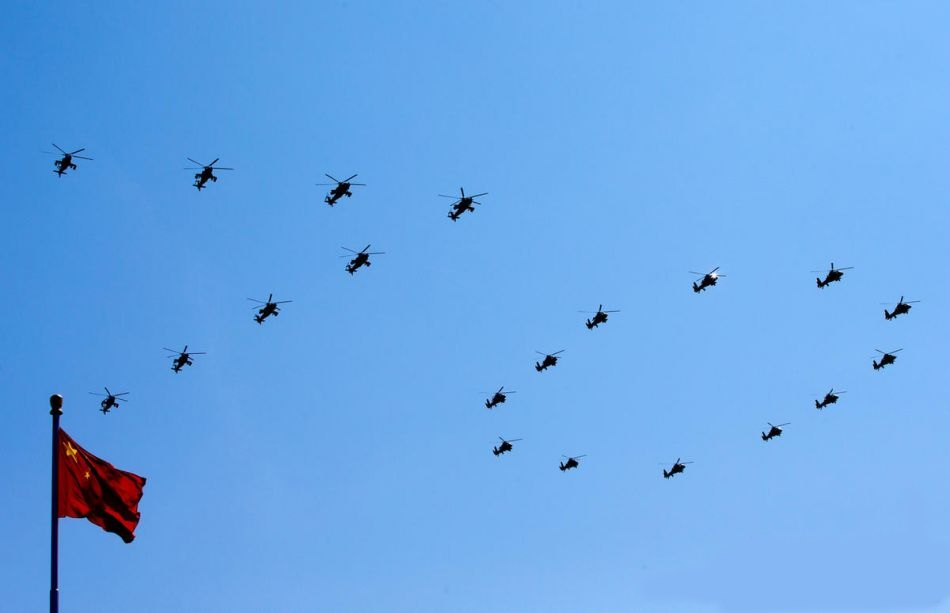
\includegraphics[width=0.23\linewidth]{picture/screenshot084}
\end{figure}


\fourchoices
{以甲为参考系,乙是运动 的}
{以乙为参考系,甲是运动的}
{以甲为参考系,坐在观众席上的观众都是静止的}
{以乙为参考系,“$ 70 $”字样编队中所有直升机都是静止的}


\item
下列说法正确的是 \xzanswer{D} 


\fourchoices
{$ \alpha $ 射线的穿透能力比 $ \beta $ 射线强}
{天然放射现象说明原子具有复杂的结构}
{核聚变中平均每个核子放出的能量比裂变中平均每个核子的小}
{半衰期跟放射性元素以单质或化合物形式存在无关}

\newpage
\item
如图所示,钢球从斜槽轨道末端以 $ v_{0} $ 的水平速度飞出,经过时间 $ t $ 落在斜靠的挡板 $ AB $ 中点。若钢球以 $ 2 v_{0} $
的速度水平飞出,则 \xzanswer{C} 
\begin{figure}[h!]
\centering
\includesvg[width=0.23\linewidth]{picture/svg/GZ-3-tiyou-0678}
\end{figure}

\fourchoices
{下落时间仍为 $ t $}
{下落时间为 $ 2t $}
{下落时间为 $ \sqrt{2} t $}
{落在挡板底端 $ B $ 点}



\item
小明在一根细橡胶管中灌满食盐水,两端用粗铜丝塞住管口,形成一段封闭的盐水柱。他将此盐水柱接
到电源两端,电源电动势和内阻恒定。握住盐水柱两端将它水平均匀拉伸到原长的 $ 1.2 $ 倍,若忽略温度对电
阻率的影响,则此盐水柱 \xzanswer{B} 


\fourchoices
{通过的电流增大}
{两端的电压增大}
{阻值增大为原来的 $ 1.2 $ 倍}
{电功率增大为原来的 $ 1.44 $ 倍}


\item
如图所示,电子以某一初速度沿两块平行板的中线方向射入偏转电场中,已知极板长度 $ l $,间距 $ d $,电子
质量 $ m $,电荷量 $ e $。若电子恰好从极板边缘射出电场,由以上条件可以求出的是 \xzanswer{B} 
\begin{figure}[h!]
\centering
\includesvg[width=0.3\linewidth]{picture/svg/GZ-3-tiyou-0679}
\end{figure}


\fourchoices
{偏转电压}
{偏转的角度}
{射出电场速度}
{电场中运动的时间}


\item
如图所示,单刀双掷开关 $ S $ 先打到 $ a $ 端让电容器充满电。 $ t=0 $ 时开关 $ S $ 打到 $ b $ 端, $ t=0.02 \ s $ 时 $ LC $ 回路
中电容器下极板带正电荷且电荷量第一次达到最大值。则 \xzanswer{C} 
\begin{figure}[h!]
\centering
\includesvg[width=0.3\linewidth]{picture/svg/GZ-3-tiyou-0680}
\end{figure}



\fourchoices
{$ LC $ 回路的周期为 $ 0.02 \ s $}
{$ LC $ 回路的电流最大时电容器中电场能最大}
{$ t=1.01 \ s $ 时线圈中磁场能最大}
{$ t=1.01 \ s $ 时回路中电流沿顺时针方向}


\item
如图所示,卫星 $ a $、$ b $、$ c $ 沿圆形轨道绕地球运行。$ a $ 是极地轨道卫星,在地球两极上空约 $ 1000 \ km $ 处运行;
$ b $ 是低轨道卫星,距地球表面高度与 $ a $ 相等;$ c $ 是地球同步卫星,则 \xzanswer{C} 
\begin{figure}[h!]
\centering
\includesvg[width=0.27\linewidth]{picture/svg/GZ-3-tiyou-1649}
\end{figure}


\fourchoices
{$ a $、$ b $ 的周期比 $ c $ 大}
{$ a $、$ b $ 的向心力一定相等}
{$ a $、$ b $ 的速度大小相等}
{$ a $、$ b $ 的向心加速度比 $ c $ 小}


\item
如图所示,甲乙两图中的理想变压器以不同的方式接在高压电路中。甲图中变压器原副线圈的匝数比为$ k_{1} $,电压表读数为 $ U $,乙图中变压器原副线圈的匝数比为 $ k_{2} $,电流表读数为$ I $。则甲图中高压线电压和乙图
中高压线电流分别为 \xzanswer{B} 
\begin{figure}[h!]
\centering
\includesvg[width=0.33\linewidth]{picture/svg/GZ-3-tiyou-0682}
\end{figure}

\fourchoices
{$k_{1} U \quad k_{2} I$}
{$ k_{1} U \quad \frac{I}{k_{2}}$}
{$\frac{U}{k_{1}} \quad k_{2} I$}
{$\frac{U}{k_{1}} \quad \frac{I}{k_{2}}$}


\item
如图所示,在光滑绝缘水平面上,两条固定的相互垂直彼此绝缘的导线通以大小相同的电流 $ I $ 。在角平
分线上,对称放置四个相同的正方形金属框。当电流在相同时间间隔内增加相同量,则 \xzanswer{B} 
\begin{figure}[h!]
\centering
\includesvg[width=0.23\linewidth]{picture/svg/GZ-3-tiyou-0683}
\end{figure}


\fourchoices
{$ 1 $、$ 3 $ 线圈静止不动,$ 2 $、$ 4 $ 线圈沿着对角线向内运动}
{$ 1 $、$ 3 $ 线圈静止不动,$ 2 $、$ 4 $ 线圈沿着对角线向外运动}
{$ 2 $、$ 4 $ 线圈静止不动,$ 1 $、$ 3 $ 线圈沿着对角线向内运动}
{$ 2 $、$ 4 $ 线圈静止不动,$ 1 $、$ 3 $ 线圈沿着对角线向外运动}


\newpage
\item
如图所示,一束光与某材料表面成 $ 45 ^{ \circ } $角入射,每次反射的光能量为入射光能量的 $ k $ 倍 $ (0<k<1) $。若
这束光最终进入材料的能量为入射光能量的 $ (1-k^{2}) $倍,则该材料折射率至少为 \xzanswer{A} 
\begin{figure}[h!]
\centering
\includesvg[width=0.23\linewidth]{picture/svg/GZ-3-tiyou-0684}
\end{figure}

\fourchoices
{$\frac{\sqrt{6}}{2}$}
{$\sqrt{2}$}
{$ 1.5 $}
{$ 2 $}


\item
如图所示,在倾角为 $ \alpha $ 的光滑绝缘斜面上固定一个挡板,在挡板上连接一根劲度系数为 $ k_{0} $ 的绝缘轻质
弹簧,弹簧另一端与 $ A $ 球连接。$ A $、$ B $、$ C $ 三小球的质量均为 $ M $, $ q_{A} =q_{0}>0 $, $ q_{B} =-q_{0} $,当系统处于静
止状态时,三小球等间距排列。已知静电力常量为 $ k $,则 \xzanswer{A} 
\begin{figure}[h!]
\centering
\includesvg[width=0.23\linewidth]{picture/svg/GZ-3-tiyou-0685}
\end{figure}


\fourchoices
{$q_{\mathrm{C}}=\frac{4}{7} q_{0}$}
{弹簧伸长量为 $\frac{M g \sin \alpha}{k_{0}}$}
{A 球受到的库仑力大小为 $2 M g$}
{相邻两小球间距为 $q_{0} \sqrt{\frac{3 k}{7 M g}}$}


%二、选择题$ \lmd{2} $(本题共 $ 3 $ 小题,每小题 $ 2 $ 分,共 $ 6 $ 分。每小题列出的四个备选项中至少有一个是符合题目要求的。全部选对的得 $ 2 $ 分,选对但不全的得 $ 1 $ 分,有选错的得 $ 0 $ 分)


\item
由玻尔原子模型求得氢原子能级如图所示,已知可见光 的光子能量在 $ 1.62 \ eV $ 到 $ 3.11 \ eV $ 之间,则 \xzanswer{CD} 
\begin{figure}[h!]
\centering
\includesvg[width=0.23\linewidth]{picture/svg/GZ-3-tiyou-0686}
\end{figure}


\fourchoices
{氢原子从高能级向低能级跃迁时可能辐射出 $ \gamma $ 射线}
{氢原子从 $ n=3 $ 的能级向 $ n=2 $ 的能级跃迁时会辐射出红外线}
{处于 $ n=3 $ 能级的氢原子可以吸收任意频率的紫外线并发生电离}
{大量氢原子从 $ n=4 $ 能级向低能级跃迁时可辐射出 $ 2 $ 种频率的可见光}



\item
如图所示,波长为 $ \lambda_{a} $ 和 $ \lambda_{b} $ 的两种单色光射入三棱镜,经折射后射出两束单色光 $ a $ 和 $ b $,则这两束光 \xzanswer{BD} 
\begin{figure}[h!]
\centering
\includesvg[width=0.17\linewidth]{picture/svg/GZ-3-tiyou-1648}
\end{figure}


\fourchoices
{照射同一种金属均有光电子逸出,光电子最大初动能 $ E_{Ka}>E_{Kb} $}
{射向同一双缝干涉装置,其干涉条纹间距 $ \Delta x_a> \Delta x_b $}
{在水中的传播速度 $ v_a<v_b $}
{光子动量 $ p_a<p_b $}


\item
如图所示,波源 $ O $ 垂直于纸面做简谐运动,所激发的横波在均匀介质中向四周传播,图中虚线表示两个
波面。 $ t=0 $ 时,离 $ O $ 点 $ 5 \ m $ 的 $ A $ 点开始振动; $ t=1 \ s $ 时,离 $ O $ 点 $ 10 \ m $ 的 $ B $ 点也开始振动,此时 $ A $ 点第五次
回到平衡位置,则 \xzanswer{AB} 
\begin{figure}[h!]
\centering
\includesvg[width=0.23\linewidth]{picture/svg/GZ-3-tiyou-0688}
\end{figure}

\fourchoices
{波的周期为 $ 0.4 \ s $}
{波的波长为 $ 2 \ m $}
{波速为 $ 5\sqrt{3} \ m/s $}
{$ t=1 \ s $ 时 $ AB $ 连线上有 $ 4 $ 个点处于最大位移}



%三、非选择题(本题共 $ 6 $ 小题,共 $ 55 $ 分)

\gaokaosy


\item
在“探究加速度与力、质量的关系”和用橡皮筋“探究做功与物体速度变化的关系”实验中:
\begin{enumerate}
%\renewcommand{\labelenumi}{\arabic{enumi}.}
% A(\Alph) a(\alph) I(\Roman) i(\roman) 1(\arabic)
%设定全局标号series=example	%引用全局变量resume=example
%[topsep=-0.3em,parsep=-0.3em,itemsep=-0.3em,partopsep=-0.3em]
%可使用leftmargin调整列表环境左边的空白长度 [leftmargin=0em]
\item
都是通过分析纸带上的点来测量物理量,下列说法正确的是 \underlinegap .

\fourchoices
{都需要分析打点计时器打下的第一个点}
{都不需要分析打点计时器打下的第一个点}
{一条纸带都只能获得一组数据}
{一条纸带都能获得多组数据}


\item 
如图是两条纸带的一部分,$ A $、$ B $、$ C $、$ \cdots $、$ G $ 是纸带上标出的计数点,每两个相邻的计数点之间还有
$ 4 $个打出的点未画出。其中图 \underlinegap (填“$ a $”或“$ b $”)所示的是用橡皮筋“探究做功与物体速度变化的
关系”的实验纸带。“探究加速度与力、质量的关系”实验中,小车的加速度大小 $ a=$ \underlinegap $m/s^{2} $(保留 $ 2 $ 位有效数字)。
\begin{figure}[h!]
\centering
\begin{subfigure}{0.7\linewidth}
\centering
%\includesvg[width=0.9\linewidth]{picture/svg/GZ-3-tiyou-0689}
 \includesvg[width=0.9\linewidth]{picture/svg/GZ-3-tiyou-1646} 
\caption{}\label{}
\end{subfigure}
\begin{subfigure}{0.7\linewidth}
\centering
%\includesvg[width=0.9\linewidth]{picture/svg/GZ-3-tiyou-0690}
 \includesvg[width=0.93\linewidth]{picture/svg/GZ-3-tiyou-1647} 
\caption{}\label{}
\end{subfigure}

\end{figure}



\item 
在用橡皮筋“探究做功与物体速度变化的关系”实验中,平衡阻力后,小车与橡皮筋组成的系统在橡
皮筋恢复形变前机械能 \underlinegap (填“守恒”或“不守恒”)。


\end{enumerate}



\tk{
\begin{enumerate}
%\renewcommand{\labelenumi}{\arabic{enumi}.}
% A(\Alph) a(\alph) I(\Roman) i(\roman) 1(\arabic)
%设定全局标号series=example	%引用全局变量resume=example
%[topsep=-0.3em,parsep=-0.3em,itemsep=-0.3em,partopsep=-0.3em]
%可使用leftmargin调整列表环境左边的空白长度 [leftmargin=0em]
\item
BC
\item 
$ a $
\item 
$ 0.40 $
\item 
不守恒
\end{enumerate}
} 

\item 
\begin{enumerate}
%\renewcommand{\labelenumi}{\arabic{enumi}.}
% A(\Alph) a(\alph) I(\Roman) i(\roman) 1(\arabic)
%设定全局标号series=example	%引用全局变量resume=example
%[topsep=-0.3em,parsep=-0.3em,itemsep=-0.3em,partopsep=-0.3em]
%可使用leftmargin调整列表环境左边的空白长度 [leftmargin=0em]
\item
小明同学用多用电表测量一未知电阻器的阻值。经过规范操作后,所选欧姆挡倍率及指针位置分
别如图$ a $、$ b $所示,则此电阻器的阻值为 \underlinegap $ \Omega $。
\begin{figure}[h!]
\centering
\begin{subfigure}{0.4\linewidth}
\centering
%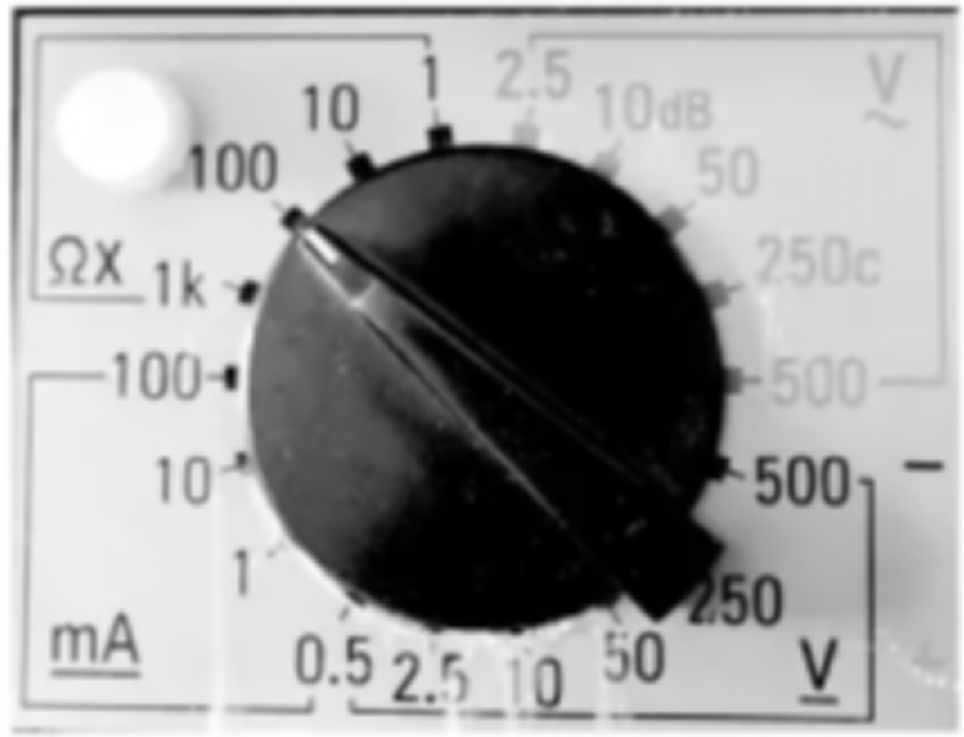
\includegraphics[width=0.7\linewidth]{picture/screenshot036}
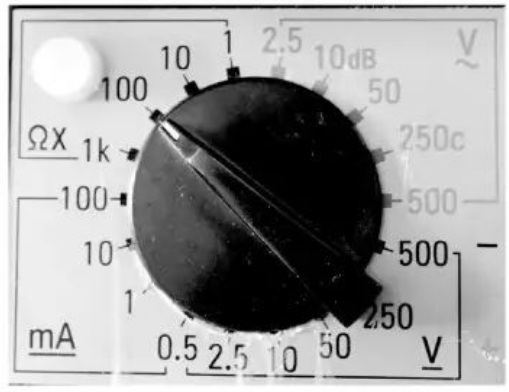
\includegraphics[width=0.7\linewidth]{picture/screenshot090}
\caption{}\label{}
\end{subfigure}
\begin{subfigure}{0.4\linewidth}
\centering
%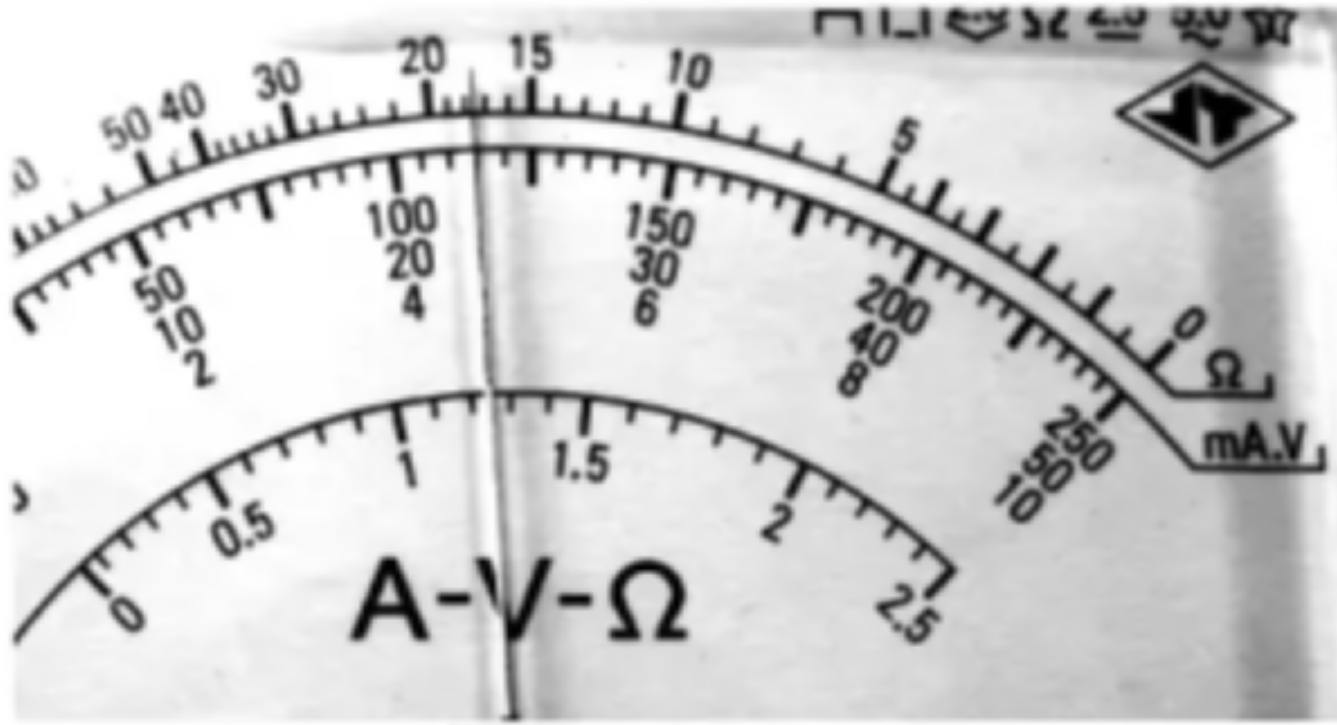
\includegraphics[width=0.7\linewidth]{picture/screenshot037}
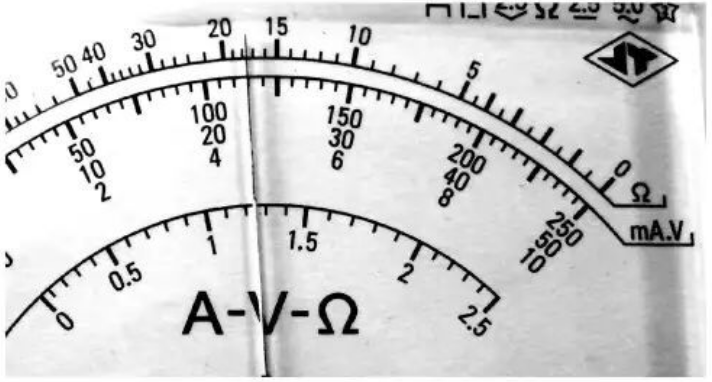
\includegraphics[width=0.8\linewidth]{picture/screenshot091}
\caption{}\label{}
\end{subfigure}
\begin{subfigure}{0.4\linewidth}
\centering
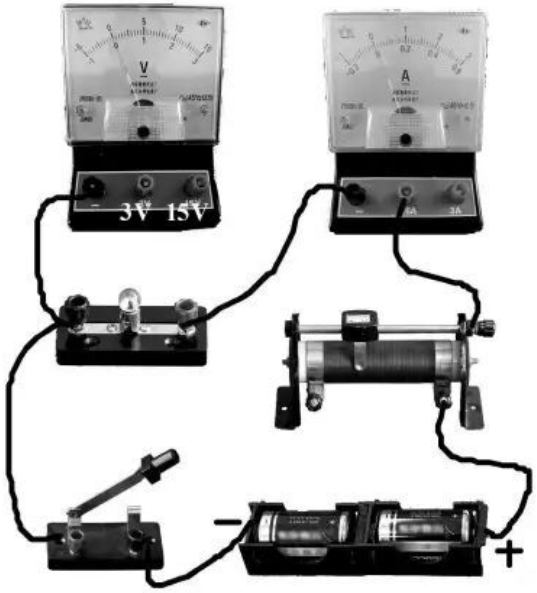
\includegraphics[width=0.7\linewidth]{picture/screenshot089}
\caption{}\label{}
\end{subfigure}
\begin{subfigure}{0.4\linewidth}
\centering
%\includesvg[width=0.8\linewidth]{picture/svg/GZ-3-tiyou-0692}
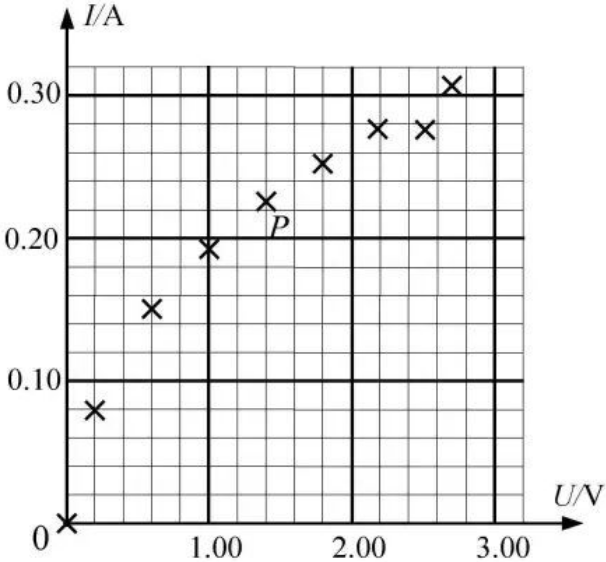
\includegraphics[width=0.8\linewidth]{picture/screenshot088}
\caption{}\label{}
\end{subfigure}
\end{figure}




\item 
在“测绘小灯泡 的伏安特性曲线”实验中:
\begin{enumerate}
	%\renewcommand{\labelenumi}{\arabic{enumi}.}
	% A(\Alph) a(\alph) I(\Roman) i(\roman) 1(\arabic)
	%设定全局标号series=example	%引用全局变量resume=example
	%[topsep=-0.3em,parsep=-0.3em,itemsep=-0.3em,partopsep=-0.3em]
	%可使用leftmargin调整列表环境左边的空白长度 [leftmargin=0em]
	\item
如图$ c $所示,已经连接了一部分电路,请在答题纸上对应位置将电路连接完整。


\item 
合上开关后,测出 $ 9 $ 组$ \lmd{1} $、$ U $ 值,在 $ I-U $ 坐标系中描出各对应点,如图$ d $所示。请在答题纸对应位置的
图中画出此小灯泡的伏安特性曲线。


\item 
与图$ d $中 $ P $ 点对应的状态,小灯泡灯丝阻值最接近 \underlinegap 。
\threechoices
{$ 16.7 \ \Omega $}
{$ 12.4 \ \Omega $}
{$ 6.2 \ \Omega $}

\end{enumerate}


\end{enumerate}

\tk{
\begin{enumerate}
%\renewcommand{\labelenumi}{\arabic{enumi}.}
% A(\Alph) a(\alph) I(\Roman) i(\roman) 1(\arabic)
%设定全局标号series=example	%引用全局变量resume=example
%[topsep=-0.3em,parsep=-0.3em,itemsep=-0.3em,partopsep=-0.3em]
%可使用leftmargin调整列表环境左边的空白长度 [leftmargin=0em]
\item
$1750(1700 \sim 1800)$	
\item 
如图
\begin{center}
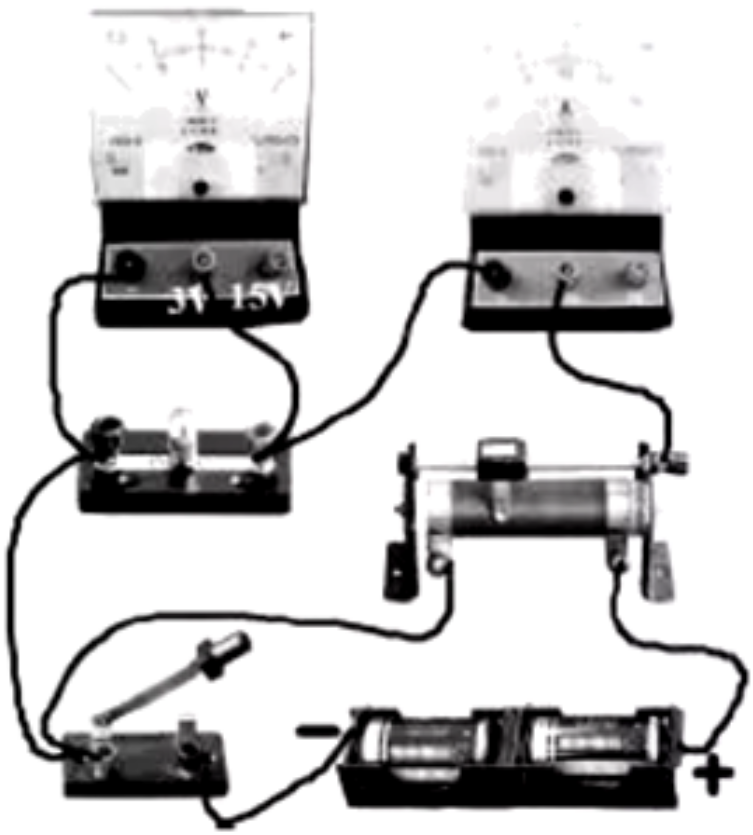
\includegraphics[width=0.7\linewidth]{picture/screenshot040}
\end{center}
\begin{center}
 \includesvg[width=0.7\linewidth]{picture/svg/GZ-3-tiyou-0697} 
\end{center}
\item 
C
\end{enumerate}
} 


\newpage

\gaokaojs

\item 
一个无风晴朗的冬日,小明乘坐游戏滑雪车从静止开始沿斜直雪道下滑,滑行 $ 54 \ m $ 后进入水平雪道,
继续滑行 $ 40.5 \ m $ 后减速到零。已知小明和滑雪车的总质量为 $ 60 \ kg $,整个滑行过程用时 $ 10.5 \ s $,斜直雪道倾角
为 $ 37 ^{ \circ } (\sin 37 \degree =0.6) $。求小明和滑雪车:
\begin{enumerate}
%\renewcommand{\labelenumi}{\arabic{enumi}.}
% A(\Alph) a(\alph) I(\Roman) i(\roman) 1(\arabic)
%设定全局标号series=example	%引用全局变量resume=example
%[topsep=-0.3em,parsep=-0.3em,itemsep=-0.3em,partopsep=-0.3em]
%可使用leftmargin调整列表环境左边的空白长度 [leftmargin=0em]
\item
滑行过程中的最大速度 $ v_{m} $ 的大小;
\item 
在斜直雪道上滑行的时间 $ t_{1} $;
\item 
在斜直雪道上受到的平均阻力 $ F_{f} $ 的大小。

\end{enumerate}
% TODO: \usepackage{graphicx} required
\begin{figure}[h!]
\flushright 
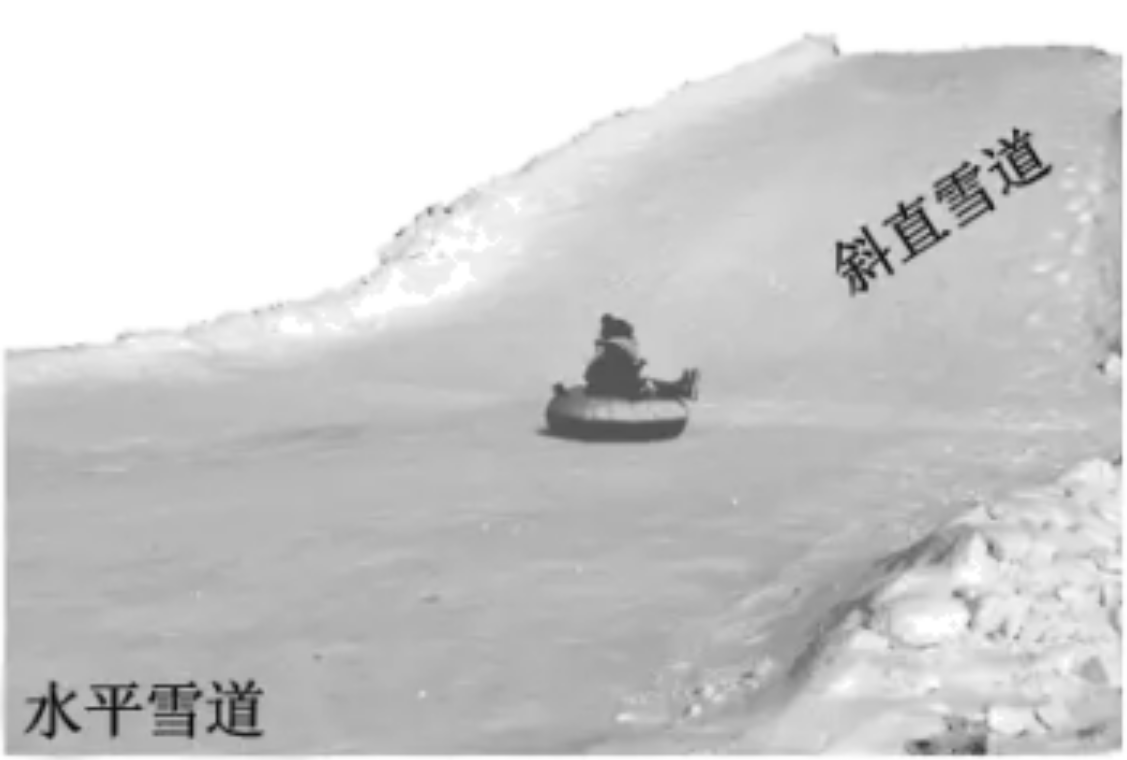
\includegraphics[width=0.23\linewidth]{picture/screenshot039}
\end{figure}


\banswer{
\begin{enumerate}
%\renewcommand{\labelenumi}{\arabic{enumi}.}
% A(\Alph) a(\alph) I(\Roman) i(\roman) 1(\arabic)
%设定全局标号series=example	%引用全局变量resume=example
%[topsep=-0.3em,parsep=-0.3em,itemsep=-0.3em,partopsep=-0.3em]
%可使用leftmargin调整列表环境左边的空白长度 [leftmargin=0em]
\item
$v_{m}=18 \ m/s$
\item 
$t_{1}=6 \ s $
\item 
$ F_{f}=180 \ N$
\end{enumerate}
}


\item
如图所示,一弹射游戏装置由安装在水平台面上的固定弹射器、竖直圆轨道(在最低点 $ E $ 分别与水平轨道 $ EO $ 和 $ EA $ 相连)、高度 $ h $ 可调的斜轨道 $ AB $ 组成。游戏时滑块从 $ O $ 点弹出,经过圆轨道并滑上斜轨道。
全程不脱离轨道且恰好停在 $ B $ 端则视为游戏成功。已知圆轨道半径 $ r=0.1 \ m $, $ OE $ 长 $ L_{1} =0.2 \ m $, $ AC $ 长
$ L_{2} =0.4 \ m $,圆轨道和 $ AE $ 光滑,滑块与 $ AB $、 $ OE $ 之间的动摩擦因数 $ \mu=0.5 $。滑块质量 $ m=2 \ g $ 且可视为
质点,弹射时从静止释放且弹簧的弹性势能完全转化为滑块动能。忽略空气阻力,各部分平滑连接。求:
\begin{enumerate}
%\renewcommand{\labelenumi}{\arabic{enumi}.}
% A(\Alph) a(\alph) I(\Roman) i(\roman) 1(\arabic)
%设定全局标号series=example	%引用全局变量resume=example
%[topsep=-0.3em,parsep=-0.3em,itemsep=-0.3em,partopsep=-0.3em]
%可使用leftmargin调整列表环境左边的空白长度 [leftmargin=0em]
\item
滑块恰好能过圆轨道最高点 $ F $ 时的速度 $ v_F $ 大小;
\item 
当 $ h=0.1 \ m $ 且游戏成功时,滑块经过 $ E $ 点对圆轨道的压力 $ F_{N} $ 大小及弹簧的弹性势能 $ E_{p0} $;
\item 
要使游戏成功,弹簧的弹性势能 $ E_{P} $ 与高度 $ h $ 之间满足的关系。

\end{enumerate}
\begin{figure}[h!]
\flushright
\includesvg[width=0.45\linewidth]{picture/svg/GZ-3-tiyou-0693}
\end{figure}


\banswer{
\begin{enumerate}
%\renewcommand{\labelenumi}{\arabic{enumi}.}
% A(\Alph) a(\alph) I(\Roman) i(\roman) 1(\arabic)
%设定全局标号series=example	%引用全局变量resume=example
%[topsep=-0.3em,parsep=-0.3em,itemsep=-0.3em,partopsep=-0.3em]
%可使用leftmargin调整列表环境左边的空白长度 [leftmargin=0em]
\item
$v_{F}=1 \ m / s$
\item 
$E_{p 0}=8.0 \times 10^{-3} \ J$
\item 
$ 	E_{p}=m g h+\mu m g\left(L_{1}+L_{2}\right)  $\\
$ E_{p}=2 \times 10^{-3}(10 h+3) \ J $
\end{enumerate}
}



\newpage
\item
如图甲所示,在 $ xOy $ 水平面内,固定放置着间距为 $ l $ 的两平行金属直导轨,其间连接有阻值为 $ R $ 的电阻,
电阻两端连接示波器(内阻可视为无穷大),可动态显示电阻 $ R $ 两端的电压。两导轨间存在大小为 $ B $、方向
垂直导轨平面的匀强磁场。 $ t=0 $ 时一质量为 $ m $、长为 $ l $ 的导体棒在外力 $ F $ 作用下从 $ x=x_{0} $位置开始做简
谐运动,观察到示波器显示的电压随时间变化的波形是如图乙所示的正弦曲线。取 $x_{0}=-\frac{U_{m} T}{2 \pi B l}$,则简谐运
动的平衡位置在坐标原点 $ O $。不计摩擦阻力和其它电阻,导体棒始终垂直导轨运动。
(提示:可以用 $ F-x $ 图
象下的“面积”代表力 $ F $ 所做的功)
\begin{enumerate}
%\renewcommand{\labelenumi}{\arabic{enumi}.}
% A(\Alph) a(\alph) I(\Roman) i(\roman) 1(\arabic)
%设定全局标号series=example	%引用全局变量resume=example
%[topsep=-0.3em,parsep=-0.3em,itemsep=-0.3em,partopsep=-0.3em]
%可使用leftmargin调整列表环境左边的空白长度 [leftmargin=0em]
\item
求导体棒所受到的安培力 $ F_{A} $ 随时间 $ t $ 的变化规律;
\item 
求在 $ 0 $ 至 $ 0.25 \ T $ 时间内外力 $ F $ 的冲量;
\item 
若 $ t=0 $ 时外力 $ F_0=1 \ N,l=1 \ m,T=2 \pi \ s,m=1 \ kg,R=1 \ \Omega ,U_{m}=0.5 \ V ,B=0.5 \ T $,求外力与安培力大
小相等时棒的位置坐标和速度。

\end{enumerate}
\begin{figure}[h!]
\flushright 
\begin{subfigure}{0.4\linewidth}
\centering
\includesvg[width=0.9\linewidth]{picture/svg/GZ-3-tiyou-0694} 
\caption{}\label{}
\end{subfigure}
\begin{subfigure}{0.4\linewidth}
\centering
\includesvg[width=0.85\linewidth]{picture/svg/GZ-3-tiyou-0695} 
\caption{}\label{}
\end{subfigure}	
\end{figure}


\banswer{
\begin{enumerate}
%\renewcommand{\labelenumi}{\arabic{enumi}.}
% A(\Alph) a(\alph) I(\Roman) i(\roman) 1(\arabic)
%设定全局标号series=example	%引用全局变量resume=example
%[topsep=-0.3em,parsep=-0.3em,itemsep=-0.3em,partopsep=-0.3em]
%可使用leftmargin调整列表环境左边的空白长度 [leftmargin=0em]
\item
$-\frac{B l U_{m}}{R} \sin \frac{2 \pi}{T} t$
\item 
$I_{F}=\frac{B l U_{m} T}{2 \pi R}+\frac{m U_{m}}{B l}$
\item 
\begin{enumerate}
	%\renewcommand{\labelenumi}{\arabic{enumi}.}
	% A(\Alph) a(\alph) I(\Roman) i(\roman) 1(\arabic)
	%设定全局标号series=example	%引用全局变量resume=example
	%[topsep=-0.3em,parsep=-0.3em,itemsep=-0.3em,partopsep=-0.3em]
	%可使用leftmargin调整列表环境左边的空白长度 [leftmargin=0em]
	\item
当 $F_{A}=-F$ 时\\
 $ x=0, v=\pm v_{in}=\pm 1\ m / s$
\item 
当 $F_{A}=F$ 时\\
$x_{1}^{\prime}=\frac{1}{\sqrt{5}} \ m$ 和 $v_{1}^{\prime}=\frac{2}{\sqrt{5}} \ m / s $\\ 
$ x_{2}^{\prime}=-\frac{1}{\sqrt{5}} \ m$ 和 $v_{2}^{\prime}=-\frac{2}{\sqrt{5}} \ m$
\end{enumerate}
\end{enumerate}
}




\newpage

\item 
通过测量质子在磁场中的运动轨迹和打到探测板上的计数率(即打到探测板上质子数与衰变产生总质子
数 $ N $ 的比值),可研究中子( \ce{^{1}_0n} )的 $ \beta $ 衰变。中子衰变后转化成质子和电子,同时放出质量可视为零的反
中微子 $ \bar{\nu}_{e} $。如图所示,位于 $ P $ 点的静止中子经衰变可形成一个质子源,该质子源在纸面内各向均匀地发射
$ N $ 个质子。在 $ P $ 点下方放置有长度 $ L=1.2 \ m $ 以 $ O $ 为中点的探测板,$ P $ 点离探测板的垂直距离 $ OP $ 为 $ a $。在
探测板的上方存在方向垂直纸面向里,磁感应强度大小为 $ B $ 的匀强磁场。

已知电子质量 $ m_e=9.1 \times10^{-31} \ kg=0.51 \ MeV/c^{2} $,中子质量 $ m_n=939.57 \ MeV/c^{2} $,质子质量$ m_p=938.27 \ MeV/c^{2} $ ($ c $ 为光速,不考虑粒子之间的相互作用)。

若质子的动量 $ p=4.8\times10^{-21} \ kg \cdot m \cdot s^{-1}=3 \times 10^{-8} \ MeV \cdot s \cdot m^{-1} $。
\begin{enumerate}
%\renewcommand{\labelenumi}{\arabic{enumi}.}
% A(\Alph) a(\alph) I(\Roman) i(\roman) 1(\arabic)
%设定全局标号series=example	%引用全局变量resume=example
%[topsep=-0.3em,parsep=-0.3em,itemsep=-0.3em,partopsep=-0.3em]
%可使用leftmargin调整列表环境左边的空白长度 [leftmargin=0em]
\item
写出中子衰变的核反应式,求电子和反中微子的总动能(以 $ MeV $ 为能量单位);
\item 
当 $ a=0.15 \ m $, $ B=0.1 \ T $ 时,求计数率;
\item 
若 $ a $ 取不同的值,可通过调节 $ B $ 的大小获得与($ 2 $)问中同样的计数率,求 $ B $ 与 $ a $ 的关系并给出 $ B $ 的
范围。


\end{enumerate}
\begin{figure}[h!]
\flushright
\includesvg[width=0.43\linewidth]{picture/svg/GZ-3-tiyou-0696}
\end{figure}

\banswer{
\begin{enumerate}
%\renewcommand{\labelenumi}{\arabic{enumi}.}
% A(\Alph) a(\alph) I(\Roman) i(\roman) 1(\arabic)
%设定全局标号series=example	%引用全局变量resume=example
%[topsep=-0.3em,parsep=-0.3em,itemsep=-0.3em,partopsep=-0.3em]
%可使用leftmargin调整列表环境左边的空白长度 [leftmargin=0em]
\item
$ ^{1}_{0}n \rightarrow ^{1}_{1}P + ^{0}_{-1}e + ^{0}_{0} \bar{\nu_{e}} $\\
$E_{e}+E_{v}=0.7468 \ MeV$
\item 
$\eta=\frac{2}{3}$
\item 
$B=\frac{3}{200 a} \ T  \quad  (B \geqslant \frac{\sqrt{15}}{40} \ T) $
\end{enumerate}
}




\end{enumerate}

